%% LyX 2.0.3 created this file.  For more info, see http://www.lyx.org/.
%% Do not edit unless you really know what you are doing.
\documentclass[english]{article}
\usepackage{mathptmx}
\usepackage{helvet}
\usepackage{courier}
\usepackage[T1]{fontenc}
\usepackage[latin9]{inputenc}
\usepackage{geometry}
\geometry{verbose,tmargin=2.54cm,bmargin=2.54cm,lmargin=2.54cm,rmargin=2.54cm}
\usepackage{graphicx}
\usepackage{babel}
\begin{document}

\title{Finding conserved transcription factor binding sites by comparing
ChIP-seq experiments}


\author{Colin Diesh}


\date{Senior Thesis Project, Fall 2012\\
$\,$\\
First semester final report}
\maketitle
\begin{abstract}
DNA-protein interactions are essential for gene regulation, and these
interactions can be detected by using chromatin immunoprecipitation
and high throughput sequencing (ChIP-seq). Transcription factors in
particular are proteins that bind to specific sequences on the DNA,
thereby promoting or suppressing the transcription of nearby genes.
Using ChIP-seq, transcription factor binding sites are identified
as peaks in the data that represents a \textquoteleft{}tag pileup\textquoteright{}
of DNA sequences. Some binding sites have too weak of a signal to
confidently identify, but evidence from comparing ChIP-seq experiments
from the genomes of related strains may provide the additional support
needed to identify these. We found substantial evidence for weak binding
sites that are conserved but aren\textquoteright{}t found by other
peak finding algorithms, and we use a normalized difference score
described by Zheng et al (2010) to find some of these. We also introduce
a modified normalized difference score that uses data from multiple
genomes concurrently.
\end{abstract}

\section{Introduction}

The genes in our DNA are regulated by a variety of proteins that interact
and bind with the DNA. Transcription factors in particular are proteins
that can affect DNA transcription by binding to the DNA, thereby regulating
nearby genes. Transcription factors bind to a particular DNA motif,
which is a short DNA sequence that they are attracted to. Identifying
the transcription factor binding sites has become an important problem
for understanding gene regulation. However, comparisons of different
related species have shown a high degree of variability of binding
sites in human and mouse and in different strains of yeast (Odom et
al. 2003, Zheng et al. 2010). 

ChIP-seq is a next-generation sequencing method for detecting DNA-protein
interactions. ChIP-seq uses chromatin immunoprecipitation followed
by high throughput sequencing to find DNA sequences to which transcription
factors bind. ChIP-seq data is made up of many short DNA sequences,
and after the sequences are aligned to a reference genome, the transcription
factor binding sites appear as \textquoteleft{}peaks\textquoteright{}
in the data. Peak finding algorithms use a significance level that
is based on a somewhat arbitrary threshold. 

In order to compare ChIP-seq data, typically, the binding sites from
different experiments are identified from each experiment individually,
and if the location of a binding sites overlap at the same genome
position in each experiment, then they are shared. If the comparison
involves comparing different genomes, then we can either compare nearby
genes of the binding sites if there exist homologous genes to compare.
Other techniques for comparing binding sites from different genomes
use a DNA alignment of each genome to find overlapping binding sites.
Odom et al. (2007) developed a peak classification that uses DNA alignment
and the ChIP signal to compare human and mouse binding sites which
illustrates how binding sites can vary from comparing different genomes.

Using the peak classification, conserved binding sites are defined
as binding sites that have the same target gene which also have conserved
DNA alignments. The conserved DNA alignment is typically characterized
using motif finding (Odom et al. 2007) but they can also use multiple
sequence alignments (Moses et al. 2004). A gained or lost peak will
have conserved sequences, but they will not have similar peak characteristics.
The unaligned and turnover classes of peaks will not have a matching
the sequence alignment, \textquotedblleft{}so they can not be classified
definitely\textquotedblright{} (Odom et al. 2007).

\begin{figure}


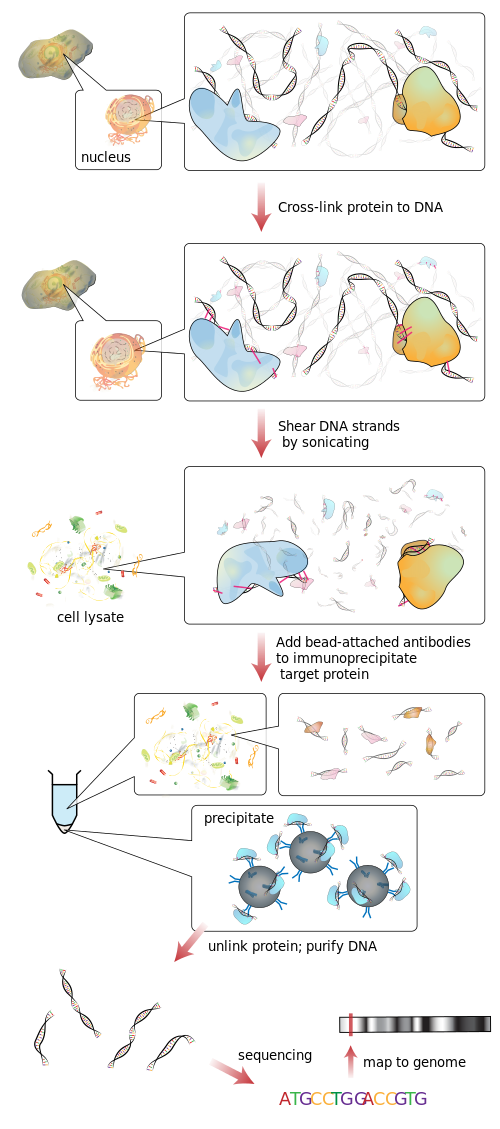
\includegraphics[scale=0.6]{image1}

\caption{Peak classification uses a DNA alignment to classify identified binding
sites (Odom, Dowell et al, 2007)}


\end{figure}


Some binding sites have too weak of a signal to confidently identify,
but evidence from the genomes of related strains may provide the additional
support needed to identify these. Using the normalized difference
score (NormDiff) described by Zheng et al (2010), we were able to
find substantial evidence for conserved binding sites that were not
identified by MACS, a commonly-used tool for identifying binding sites
from ChIP-seq data, by comparing the NormDiff scores from peaks identified
in one experiment with the same region from another experiment (the
syntenic region). We were able to identify some additional peaks found
in one strain as conserved with a statistical analysis of the NormDiff
values. We also present modifications to the normalized difference
score that use the data from multiple genomes concurrently.


\section{Background}


\subsection{Genetic analysis of transcription factor binding variation in yeast
(Zheng et al. 2010)}

In 2010, Zheng et al. analyzed transcription factor binding sites
for Ste12, a transcription factor important in mating, for different
strains of yeast using ChIP-seq. They used a peak finding software
called MACS \textendash{} Model based analysis of ChIP-seq and they
also used a normalized difference score (see Methods) to calculate
the ChIP-seq binding signal. Then they used correlations of the binding
signal with genotypes to find the genetic factors that caused the
variations in transcription factor binding site. 


\subsection{Model based analysis of ChIP-seq (Zhang et al. 2007)}

MACS is a popular and open source software tool that is used for peak
finding ChIP-seq data. We discuss some of the details of MACS analysis
and the use of command line options for processing. MACS associates
a list of tuples corresponding to the position and orientation of
each ChIP-seq tag with each chromosome. MACS does not use any other
parts of the ChIP-seq data such as the DNA sequence or alignment quality
for processing.

To account for paired-end reads, MACS calculates a shift model that
compensates for the fact that only a part of the 5\textquoteright{}
end of the ChIP-seq fragments are sequenced. For this step, MACS uses
a \textquotedblleft{}na�ve\textquotedblright{} peak finder to find
pairs of peaks on each strand within a scanning window, and then calculates
the median distance between each pair to estimate the total ChIP-seq
fragment size. Then MACS extends each read towards the 3\textquoteright{}
end to represent the true length of the ChIP-seq fragments for downstream
analysis.

For finding peaks, MACS uses a Poisson distribution model to find
data that is highly different from the background distribution. The
rate parameter of the Poisson is calculated as the expected number
of reads in the scanning window given the total number of reads and
the whole genome size. Then peaks are identified as the Poisson CDF
likelihood of receiving a large number of reads in our scan window
given the Poisson rate of the background. Poisson rate parameters
are also estimated for local 5k and 10k windows surrounding the scanning
window in order to capture local variations in the data that might
affect peak finding. 

Finally, MACS gives us the list of high quality potential transcription
factor binding sites. In the next sections, we show our methods for
comparing the data from multiple experiments to find conserved transcription
factor binding sites.

\includegraphics[scale=0.5]{Poisson_cdf}

Figure 1. The Poisson cumulative distribution function (CDF) outputs
a probability for observing a given number of events.\\



\subsection{Finding conserved transcription factor binding sites}

Finding conserved binding sites from different experiments is important
for measuring data similarity, experimental reproducibility, and finding
biological invariants in different experiments. However, ChIP-seq
experiments are subject to many variables such as noise, bias, and
differences in sequencing depth (Shao et al. 2012). These variables
can make comparing different ChIP-seq experiments difficult, so it
is important to find a good model for comparing the datasets. 

A conserved binding site can be identified by overlapping the peaks
and we can compare data about the fold-enrichment of the peak over
the background, the p-values for the distribution, and the empirical
false discovery rate can also be used to assess the binding site similarity.
However, if we want to find weakly conserved binding sites, then using
a low significance threshold for MACS can result in many false positives.
Therefore we developed a method for finding shared binding sites from
multiple experiments by comparing the normalized difference score
from the peaks that MACS identifies in one experiment to find peaks
that aren\textquoteright{}t identified in other experiments.


\section{Approach}

In order to compare different ChIP-seq experiments and find conserved
binding sites, we use a normalized difference (NormDiff) score to
calculate the \textquotedblleft{}background subtracted\textquotedblright{}
and normalized ChIP-seq binding signal. We used MACS to find high
confidence peaks from both ChIP-seq datasets, and we then we used
the normalized difference score to compare the peaks identified in
one experiment with the same region from another experiment (the syntenic
region). 

We used the number of ChIP-seq tags that overlap each genome position
to calculate the normalized difference score for each genome position
(see Methods). Then we used a sliding window to calculate the maximum
average NormDiff score for the region syntenic to each peak. We found
that many peaks NormDiff overlap in the syntenic regions, corresponding
with enriched ChIP-seq binding signal (Figure 3). Using the normal
distribution of the NormDiff scores, we calculated shared binding
sites from NormDiff scores as a statistical likelihood that the peak
is different from the background.\\


\includegraphics[scale=0.3]{Rplot02_2}\includegraphics[scale=0.3]{Rplot03}

Figure 2. The maximum average NormDiff score of peaks shared binding
sites is colored red but unique binding sites identified in only one
experiment are colored blue/green


\subsection{Results}

We found 42 new binding sites in HS959 with that were conserved in
S96 that were not identified by MACS with P<0.05, and 4 of binding
sites that were conserved with P<0.01. We also found 76 binding sites
in S96 with P<0.05 that were conserved in HS959, and 13 of these binding
sites were conserved with P<0.01 

To evaluate the significance of these findings, we evaluated all binding
sites from S96 and identified 98\% (885/897) using our method at P<0.05,
and 60\% (563/897) binding sites at a P<0.01. In HS959 we identified
85\% (729/824) of the same binding sites at P<0.05 and 46\% (365/824)
at P<0.01\\


\includegraphics[scale=0.3]{Rplot23}\includegraphics[scale=0.3]{Rplot25_2}\\
Figure 3. The maximum average NormDiff score is used to identify additional
binding sites that are conserved in each experiment. 


\section{Discussion}

Using our method there appeared to be evidence for conserved binding
sites that were not identified by other peak finding algorithms. We
found a significant enrichment of NormDiff scores for many binding
sites, which represents strong binding signals, even for binding sites
that were not identified as shared by MACS. Peaks that were not identified
by MACS but for which there might still be shared peaks, we call the
\textquotedblleft{}twilight zone\textquotedblright{}.\\


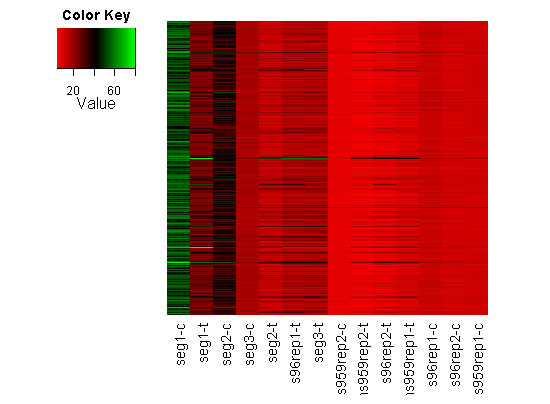
\includegraphics[scale=0.3]{image11}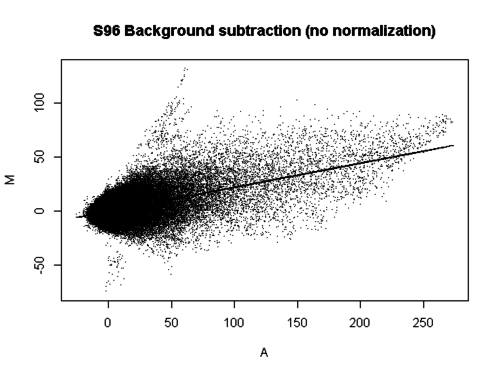
\includegraphics[scale=0.3]{image12}

Figure 4. The twilight zone in yellow shows where the normalized difference
scores from each experiment overlap significantly \\


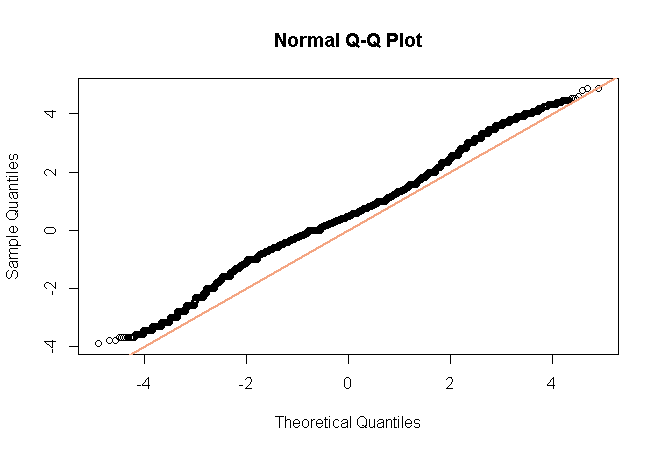
\includegraphics[scale=0.3]{image16}

Figure 5. A shared binding sites that we identified using our algorithm
has the above distribution.\\


Our work could be extended to use more sophisticated statistical models
for NormDiff too. For example, we considered modifying NormDiff scores
to use data from multiple experiments in order to find conserved binding
sites. We also discuss some of the drawbacks of our method, and the
other applications of NormDiff. 


\subsection{Modified normdiff score}

We propose using a modified NormDiff score that uses data from multiple
experiments. A NormDiff score that adds data from two experiments,
A1,B1,A2, and B2 can be defined as \\
\[
Z_{add}(x_{i})=\frac{(A_{1}-B_{1}/c_{1})+(A_{2}-B_{2}/c_{2})}{\sigma}
\]


Then the scaling factors $c_{1}$and $c_{2}$ are estimated from data,
and the variance is $\sigma=\sqrt{A_{1}+B_{1}/c_{1}^{2}+A_{2}+B_{2}/c{}_{2}^{2}}$ 

A NormDiff score that subtracts data from two experiments could also
be defined as
\[
Z_{sub}(x_{i})=\frac{(A_{1}-B_{1}/c_{1})-(A_{2}-B_{2}/c_{2})}{\sigma}
\]


The variance for $Z_{sub}$ would be the same as the variance for
$Z_{add}$. It is possible that adding and subtracting NormDiff scores
might be able to help in identifying conserved and differential binding.
For example, if the subtractive score is small but the additive score
is large, then the binding site is likely to be conserved in both
experiments. This method is similar to an MA plot which compares the
log-product and log-ratio of two experiments, however, our method
does not exaggerate small changes like the log-scale does.\\


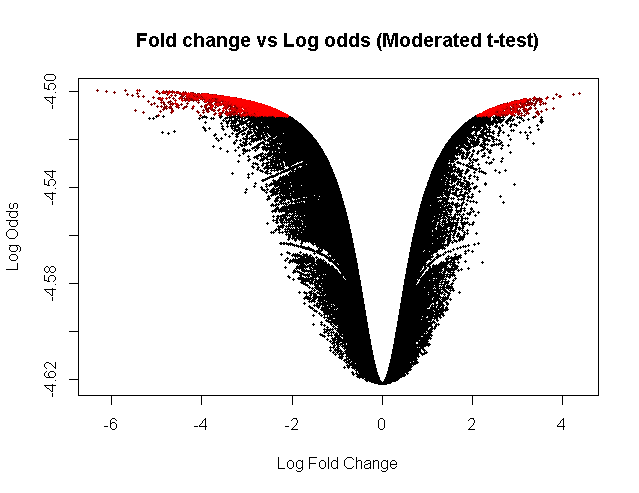
\includegraphics[scale=0.3]{image25}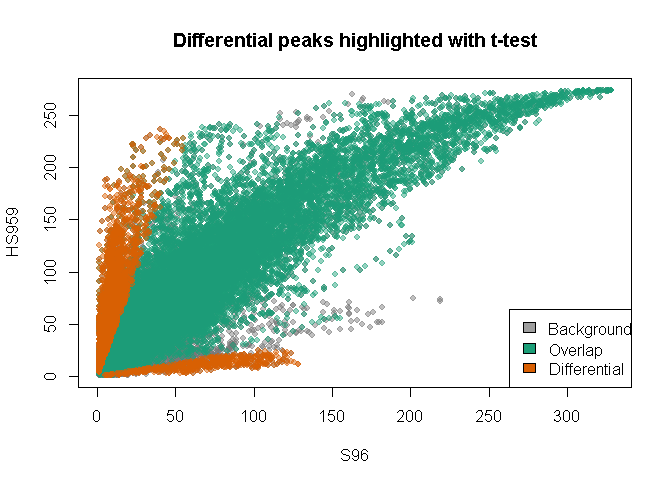
\includegraphics[scale=0.3]{image26}

Figure 6. $Z_{add}$ vs. $Z_{sub}$ for S96 and HS959. The modified
NormDiff scores are used to find evidence of shared binding sites
in the HS959 and S96 genomes. Both genomes are considered concurrently
with the modified NormDiff score to find shared peaks

\includegraphics[scale=0.3]{Rplot05}

Figure 7. MA-plot of shared and unique peaks from S96 and HS959. Unique
peaks to S96 colored green, unique peaks to HS959 colored red, shared
peaks from both colored blue.

.


\subsection{Drawbacks of our approach}

Our approach tries to find evidence for conserved binding sites by
analyzing data using normalized difference scores. Our approach gives
some evidence of peaks with high confidence P-values, such as our
results of finding new peaks with P<0.01. However, these findings
have much less confidence than thresholds set by MACS (P<1e-5). Given
that our technique for calculating P-value is similar to MACS, i.e.
by finding deviations from the background, our results are not very
strong. 

One of the reasons that we have less confidence in P-values is because
NormDiff uses control data for background subtraction. MACS does not
use control data to calculate P-values, but it uses control data to
calculate false discovery rates. Additionally, we use a normal approximation
for our data, but since our data is not continuous it may not behave
as well as Poisson distribution. 


\section{Conclusion}

We found a method for comparing binding sites from different ChIP-seq
experiments by using a normalized difference score. This gave us evidence
for shared binding sites that were not called by other peak finding
algorithms. While it was able to produce some evidence, the confidence
levels were much less than MACS which presented a challenge to the
conclusions we could make. Despite these issues, NormDiff is a powerful
tool for analyzing ChIP-seq data in other ways. NormDiff effectively
models the ChIP-seq binding signal and it can be used to compare ChIP-seq
data across multiple experiments


\section{Methods}


\subsection{Normalized difference scores}

The normalized difference (NormDiff) score is a useful statistic for
comparing ChIP-seq data that uses background subtraction and normalization
to obtain the ChIP-seq binding signal. The NormDiff score from Zheng
et al. uses a simple random model for ChIP-seq ($A$) and control
($B$) defined as

\begin{eqnarray*}
A & \sim & Poisson(f+g)\\
B & \sim & Poisson(cg)
\end{eqnarray*}


Where- 

$f$ represents the binding signal

$g$ represents the background noise

$c$ is a scaling factor between $A$ and $B$\\


Then, the NormDiff $Z$ is defined for each genome position $x_{i}$
as 

\[
Z(x_{i})=\frac{A(x_{i})-B(x_{i})/c}{\sigma}
\]
 

Then the scaling factor $c$ is estimated as the median ratio of $A/B$
and the variance $\sigma$ is estimated from $\sqrt{A+B/c^{2}}$.\\


\includegraphics[scale=0.3]{Rplot08}\includegraphics[scale=0.3]{Rplot05_2}

Supplemental Figure 1. (left) Kernel density plot of NormDiff for
entire genome shows approximately normal distribution. (right) Q-Q
Plot shows that the binding signal deviates significantly from the
expected normal distribution.


\section{Bibliography}

\bibliographystyle{plain}
\nocite{*}
\bibliography{References}

\end{document}
